\documentclass[]{article}
\usepackage{amsmath}\usepackage{amsfonts}
\usepackage[margin=1in,footskip=0.25in]{geometry}
\usepackage{mathtools}
\usepackage{hyperref}
\hypersetup{
    colorlinks=true,
    linkcolor=blue,
    filecolor=magenta,
    urlcolor=cyan,
}
\usepackage[final]{graphicx}
\usepackage{listings}
\usepackage{courier}
\lstset{basicstyle=\footnotesize\ttfamily,breaklines=true}

% \usepackage{wrapfig}
\graphicspath{{.}}

\begin{document}
\begin{center}
    Class: CSE 546 \quad Name: Hongda Li \quad HW2A
\end{center}

\section*{A.0: Conceptual Questions}
    \subsection*{A.0.a}    
        False. a large value of $w_i$ can be caused by overfitting. The error will only increase if it's proven that the features of ``Number of Bathrooms'' is not having collinearity with other features, or it's the last feature that goes to zero as we increase the lambda value for Ridge Regression. 
        \\
        Another way to think about it is, assume that there is another feature says: ``The size of bath room", then in that case, this feature is essentially the same as the removed feature: ``Number of Bathrooms'', removing it will not have a huge impact on the amount of errors for the model. 
    \subsection*{A.0.b}
        The L1 norm is more likely because the derivative of $w_j$ is $\pm 1$, which means that it's not related to the actual value of $w_j$. Therefore, which ever has the most amount of reduction on the error, that $w_j$ is getting pushed to zero. 
        \\
        Or, use professor's Simon's way of doing it, the L1 Norm $||w||_1$ forms a simplex situated around the origin. If the optimal is not inside of the simplex, then the algorithm will always goes to the vertex of the simplex to optimize it, and going to the  vertex of the L1 Ball is setting one of the features to zero. 
    \subsection*{A.0.c}
        The regularizer $\sum_{i}|w|^{0.5}$ promotes sparsity because the region $\sum_{i}|w|^{0.5} = 1$ is very pointy but this is also a bad regularizer because such region is not convex, potentially given multiple solutions, or, making gradient descent slow. 
    \subsection*{A.0.d}
        True, assume it's so large thta it just shoots out of the convex region. 
    \subsection*{A.0.e}
        It works by randomly sample a batch, and we know that the sampled samples are likely to be representative of the whole sample, and in that way, the gradient computed is pointing, somewhat, in the correct direction. The dot product between the gradient given by FIRST iteration GSD and the best Gradient direction is always positive. This is true because the first iteration will always pull the $w_j$ into the range where the data is located in. 
        \\
        This is made reasonable by consider extreme choices of sample $x_i$ that gives maximal, or minimal value of predictor, and this quantity will be bounded. Hence, the first few descent step will always pull the model into that range. 
    \subsection*{A.0.f}
        SGD is faster to compute compare to GD becausit only uses a few samples but it's less likely to have a clear convergence near the optimal because it's random. 
    

\section*{A.1: Convexity and Norms}
    Here is the axioms for norms, let $x, y\in \mathbb{R}^n$, and let $||\bullet||$ be the norm operator, then it must satisfy: 
    \begin{enumerate}
    \item[1.] $\Vert x\Vert > 0$
    \item[2.] $\Vert x + y\Vert \le \Vert x\Vert + \Vert y\Vert$ 
    \item[3.] $\Vert a x\Vert = |a|\Vert x\Vert$ 
    \end{enumerate}
    \subsection*{A.1.a}
        \textbf{Objective}: Show that $f(x) = \sum_{i = 1}^{n}|x_i|$ is a norm. 
        \begin{enumerate}
            \item[1.] It's always positive because: 
                \begin{align*}\tag{A.1.a.1}\label{eqn:A.1.a.1}
                    |x_i| &\ge 0 \quad \forall 1 \le i \le n
                    \\
                    \sum_{i = 1}^{n} |x_i| &> 0
                    \\
                    \Vert x\Vert \ge 0
                \end{align*}
            \item[2.] The trianle inequality is always ture. Let's take 2 vectors $x, y \in \mathbb{R}^n$, and for each of their corresponding elements, we can apply the triangule inequality for absolute value, which is: 
            \begin{align*}\tag{A.1.a.2}\label{eqn:A.1.a.2}
                |x_i + y_i| \le& |x_i| + |y_i| \quad \forall 1\le i \le n
                \\
                \sum_{i = 1}^{n}|x_i + y_i| \le&
                \sum_{i = 1}^{n} |x_i| + \sum_{i = 1}^{n} |y_i| 
                \\
                \Vert x + y\Vert\le \Vert x\Vert + \Vert y \Vert
            \end{align*} 
            \item[3.] And the absolute scaler it's like: 
            \begin{align*}\tag{A.1.a.3}\label{eqn:A.1.a.3}
                \Vert \alpha x\Vert =&  \sum_{i = 1}^{n} |\alpha x_i|
                \\
                =& \sum_{i = 1}^{n}|\alpha||x_i| 
                \\
                =& 
                \alpha|\Vert x\Vert
            \end{align*}
        \end{enumerate}
    \subsection*{A.1.b}
        Let's consider the case when: 
        \begin{align*}\tag{A.1.b.1}\label{eqn:A.1.b.1}
            x = \begin{bmatrix}
                \frac{1}{9} \\ \frac{1}{9}
            \end{bmatrix}
            \quad 
            y = \begin{bmatrix}
                \frac{8}{9} \\ \frac{8}{9}
            \end{bmatrix}
        \end{align*}
        Then let's compute: 
        \begin{align*}\tag{A.1.b.2}\label{eqn:A.1.b.2}
            x + y =& \begin{bmatrix}
            1 \\ 1
            \end{bmatrix}
            \\
            \implies 
            \Vert x + y\Vert =& 1 +1 = 2        
        \end{align*}
        However: 
        \begin{align*}\tag{A.1.b.3}\label{eqn:A.1.b.3}
            \Vert x\Vert & = \times \left(
                \frac{2}{\sqrt{9}}
            \right)^{2} = \frac{4}{9}
            \\
            \Vert y\Vert &= \left(
                2\times\frac{2 \sqrt{2}}{3}
            \right)^2 = \left(
                \frac{4 \sqrt{2}}{2}
            \right)^2
            \\
            &= \frac{8}{81}
            \\
            \Vert x\Vert + \Vert y\Vert = \frac{44}{81} < 2 = \Vert x + y\Vert
        \end{align*}
        This is a contradiction, therefore this cannot be a way of computing norm. 
\section*{A.2}
    \subsection*{A.2.I}
        This is not convex because a the intersection of the line connecting point $b, c$ are not the whole line. A section of the line lies outside of the shaded region. 
    \subsection*{A.2.II}
        Triangle is a convex. Any line segment defined by 2 points in the triangle is inside the triangle
    \subsection*{A.2.III}
        It's not convex. Line segment connection A $a, b$ lies outside of the shape. 

\section*{A.3}
    \subsection*{A.3.a}    
        It's convex because $f(\lambda x + (1 - \lambda)y)\le \lambda f(x) + (1 - \lambda)f(y) \;\forall \lambda\in [0, 1]$ is true. All the line segment defined via 2 points on the function lies above the function, which can be easily verified graphically. 
    \subsection*{A.3.b}
        The function is not convex because $f(\frac{b + c}{2}) > \frac{1}{2}f(b) + \frac{1}{2}f(c)$. The mid point of the line segment defined by $f(b), f(c)$ below the function value at the mid point. 
    \subsection*{A.3.c}
        The midpoint of the line segment defined by $f(a), f(c)$ lies below the function evaluated at the mid point of the function. 
    \subsection*{A.3.d}
        The function III is convex on $[c,d]$. It can be verified visually.
\section*{A.4}
    This is the code for producing plots in A.4: 
    \\
    File name: ``lasso.py''
    File Content: 
    \begin{lstlisting}[language=python]
"""
This code is for CSE 546, Spring 2021, Question A4.

Author: Hongda Alto Li, Github Account: iluvjava.

Please don't copy my code cause my code is well crafted and has my style in it.

"""

import numpy as np
array = np.array
zeros = np.zeros
norm = np.linalg.norm
inf = np.inf
mean = np.mean
sum = np.sum
abs = np.abs
sign = np.sign
ones = np.ones
max = np.max
randn = np.random.randn

import matplotlib.pyplot as plt
plot = plt.plot
xscale = plt.xscale
show = plt.show
title = plt.title
xlabel = plt.xlabel
ylabel = plt.ylabel
legend = plt.legend
saveas = plt.savefig

class LassoRegression:

    def __init__(this, regularization_lambda, delta=1e-4, verbose=False):
        """
            create an instance of Lasso fit
        :param regularization_lambda:
            The lambda for L2 norm
        :param delta:
            The tolerance for measuring the convergence of the w parameter for coordinate descend.
        :param verbose:
            Whether to print out all the message when doing the coordinate descned.
        """
        this.Lambda = regularization_lambda
        this.Verbose = verbose
        this.Delta = delta
        this._weights = None
        this._b = None

    def fit(this, X, y):
        """
            Fit that data.
            NOTE: Data standardization is not used.
        :param X:
            Row data matrix. Should be n by d where n is the number of samples and d is the number of features.
        :param y:
            Label vector, strictly on dimensional.
        :return:
            This model.
        """
        assert type(X) is np.ndarray and type(y) is np.ndarray, \
            "Must use numpy array to train the lasso."
        assert len(X.shape) == 2 and len(y.shape) == 1, \
            "X must be row data matrix, 2d and y must be a 1d vector, numerical."
        assert X.shape[0] == y.shape[0], \
            "The number of rows of X must equal to the number elements in y. "
        MaxItr = 10000
        n, d   = X.shape[0], X.shape[1]
        y2d    = y[:, np.newaxis]
        deltaW = this.Delta*ones((d, 1))*1.1                   # Amount of changes for each predictor while iterating
        w      = zeros((d, 1)) if (this._weights is None) else this._weights.copy()
                                                                # !!! Use previous for optimization if model is
                                                                # asked to optimize for a second time.
        l = this.Lambda                                        # Regularizer !!!
        Itr = 0
        while norm(deltaW, inf) > this.Delta and Itr < MaxItr:
            Itr += 1
            b    = mean(y2d - X@w)     # compute offset vector.
            a    = 2*sum(X**2, axis=0) # Compuate all the k at once, because it's not related to w_k
            for k in range(d):
                a_k     = a[k]
                Indices = [J for J in range(d) if J != k]
                c_k     = 2*sum(
                                X[::, [k]]
                                *
                                (y2d - (b + X[:, Indices]@w[Indices]))
                            )
                w_k       = 0 if (abs(c_k) < l) else (c_k - sign(c_k)*l)/a_k
                deltaW[k, ...] = abs(w_k - w[k, ...])
                w[k]      = w_k
            this._print(f"delta w is: {deltaW.reshape(-1)}")
            this._print(f"lambda is: {this.Lambda}")
        if MaxItr == Itr: raise Exception("Coordinate descent Max Itr reached without converging")
        this._weights = w
        this._b = b
        return this

    def predict(this, X):
        if this.w is None:
            raise Exception("Can't predict on a lasso that is not trained yet")
        d = this.w.shape[0]
        assert d == X.shape[1], "The number of features used to predict doesn't match with what is trained on "
        return X@this.w + this.b

    @property
    def w(this):   # get the weights of the model.
        return this._weights.copy()

    @property
    def b(this):   # Get the offset of the model.
        return this._b.copy()

    def _print(this, mesg):  # print out the message if in verbose mode.
        if this.Verbose: print(mesg)


def LassoLambdaMax(X, y):
    """
        Given the samples matrix and the labels, the function reurns the minimal lambda
        such that after running the lasso algorithm, all the features model
        parameters will be set to zeros by this lambda.
    :param X:
        This is the row data matrix, n by d matrix.
    :param y:
        This is label vector, 1d vector with a length of d.
    :return:
    """
    assert type(X) is np.ndarray and type(y) is np.ndarray, \
        "Must use numpy array to train the lasso."
    assert len(X.shape) == 2 and len(y.shape) == 1, \
        "X must be row data matrix, 2d and y must be a 1d vector, numerical."
    assert X.shape[0] == y.shape[0], \
        "The number of rows of X must equal to the number elements in y. "
    y = y[:, np.newaxis]
    return max(2*abs(X.T@(y - mean(y))))


def GetLassoSyntheticTestdata(n:int, d:int, k:int, sigma=1):
    assert (n > 0) and (d > 0) and (k > 0), "n, d, k all have to be larger than zeros"
    assert k < n, "k has to be < n"
    WTruth = array([JJ/k if JJ <= k else 0 for JJ in range(1, d + 1)], dtype=np.float)[:, np.newaxis]
    Noise = np.random.randn(n, 1)*sigma
    X = randn(n, d) # std normal for best stability of the coordinate descend algorithm.
    return X, (X@WTruth + Noise).reshape(-1), WTruth


def A4a_b():

    # Part (a)
    n, d, k = 500, 1000, 100
    X, y, Wtrue = GetLassoSyntheticTestdata(n, d, k)
    LambdaMax = LassoLambdaMax(X, y)
    Ws = []
    # Feature Chosen for each lambda
    Lfc = [] # lambda and features count
    Lambda = LambdaMax
    r = 1.1
    while len(Lfc) == 0 or Lfc[-1][1] < k:
        Model = LassoRegression(regularization_lambda=Lambda)
        Model.fit(X, y)
        NonZeros = sum(Model.w != 0)
        Ws.append(Model.w)
        print(f"NonZeros: {NonZeros}")
        Lfc.append((Lambda, NonZeros))
        Lambda /= r
    plot([_[0] for _ in Lfc], [_[1] for _ in Lfc], "ko")
    xscale("log")
    xlabel(f"$\lambda$, reduction ratio: {r}")
    ylabel("Non Zeroes $w_j$")
    title("A4: Nonezeros $W_j$ vs Lambda for Lasso")
    plt.savefig("A4a-plot.png")
    show()


    # Part (b)
    # The first k elements in Wtrue is always going to be non-zeroes.
    # FDR: (Incorrect Nonzeroes in w_hat)/(total number of nonzeroes in w_hat)
    # TPR: (# of correct non-zeroes in w_har)/(k)

    WTrueNonZeroes = Wtrue != 0
    FDR = []
    TPR = []
    Lambdas = [_[0] for _ in Lfc]
    for WHat in Ws:
        WHatNonZeros = WHat != 0
        if sum(WHatNonZeros) == 0:
            Lambdas.pop(0)
            continue
        FDR.append(sum(WHatNonZeros * ~WTrueNonZeroes)/sum(WHatNonZeros))
        TPR.append(sum(WHatNonZeros[:100])/k)
    plot(Lambdas, FDR)
    plot(Lambdas, TPR)
    title("FDR vs TPR")
    xlabel("$\lambda$")
    xscale("log")
    legend(["FDR", "TPR"])
    plt.savefig("A4b-plot.png")
    show()


def main():
    def SimpleTest():
        N, d = 40, 4
        X = np.random.rand(N, d)
        Noise = np.random.randn(N, 1)*1e-3
        Wtrue = np.random.randint(0, 100, (d, 1))
        y = X@Wtrue + Noise
        y = y.reshape(-1)

        LambdaMax = LassoLambdaMax(X, y)
        print(f"LambdaMax: {LambdaMax}")

        Model = LassoRegression(regularization_lambda=LambdaMax)
        Model.fit(X, y)
        print(Model.w)
        print(Model.b)

        Model = LassoRegression(regularization_lambda=LambdaMax/2)
        Model.fit(X, y)
        print(Model.w)
        print(Model.b)

        Model = LassoRegression(regularization_lambda=0)
        Model.fit(X, y)
        print(Model.w)
        print(Model.b)
    A4a_b()


if __name__ == "__main__":
    import os
    print(f"cwd: {os.getcwd()}")
    print(f"dir: {os.curdir}")
    main()
    \end{lstlisting}
    \subsection*{A.4.a}
        Distribution use for x: 
        $$
            x_i \sim \mathbf{N}(0, 1)
        $$
        This is used because it's already standardized. I hope it works well for the purpose of the HW. 
        \\
        Reduction ratio used for lambda is: $1/1.1$
        \begin{center}
            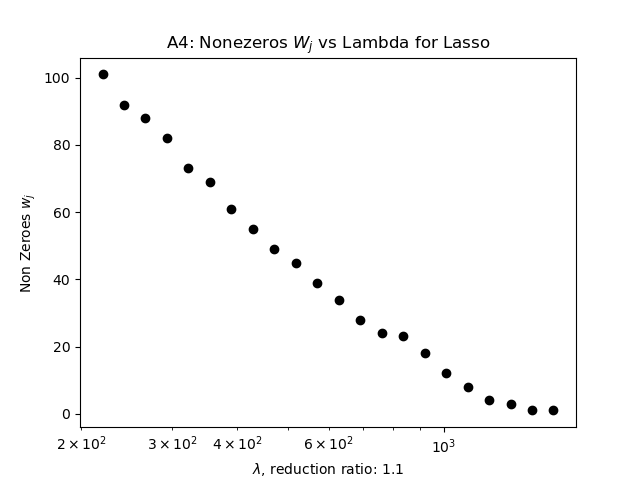
\includegraphics[width=10cm]{A4a-plot.png}
        \end{center}
        Lambda is reduced all the way until the number of non-zeroes entries went over $k$. 
    \subsection*{A.4.b}
        \begin{center}
            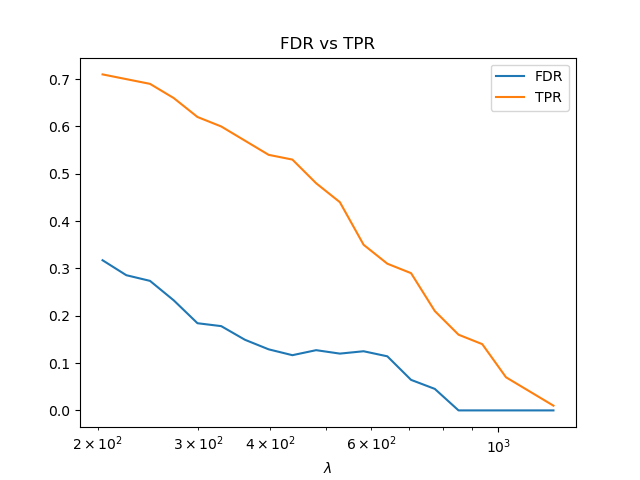
\includegraphics[width=10cm]{A4b-plot.png}
        \end{center}
        This is produced from exactly the same set of lambda and $\hat{w}^{(i)}$ with part (a) of this question for consistency. 
    \subsection*{A.4.c}
        The quantity of FDR doesn't drops to zero as the number of non-zeros terms just went over k, but it drops as we increase regularization. 
        \\
        Unfortunately, the TPR got dropped as we increase lambda as well. 
        \\
        \textbf{Note}: There are some amount of variance between different runs of the code, but the trend on the graph is mostly the same. 

\section*{A.5}
    \subsection*{A.5.a}
        \textbf{Objective}:List 3 features from the dataset that can be affected by historical policies choices. Most of the features are about populations, with a standardized measurements. 
        \\
        \begin{enumerate}
            \item[1.] There is a cluster of immigrations related features: 
                \begin{lstlisting}
    -- PctImmigRecent: percentage of _immigrants_ who immigated within last 3 years (numeric - decimal)
    -- PctImmigRec5: percentage of _immigrants_ who immigated within last 5 years (numeric - decimal)
    -- PctImmigRec8: percentage of _immigrants_ who immigated within last 8 years (numeric - decimal)
    -- PctImmigRec10: percentage of _immigrants_ who immigated within last 10 years (numeric - decimal)
    -- PctRecentImmig: percent of _population_ who have immigrated within the last 3 years (numeric - decimal)
    -- PctRecImmig5: percent of _population_ who have immigrated within the last 5 years (numeric - decimal)
    -- PctRecImmig8: percent of _population_ who have immigrated within the last 8 years (numeric - decimal)
    -- PctRecImmig10: percent of _population_ who have immigrated within the last 10 years (numeric - decimal)
                \end{lstlisting}
                These are determined by Federal Policies. 
            \item[2.] There is another cluster of police department related stats. 
            \begin{lstlisting}
-- PolicBudgPerPop: police operating budget per population (numeric - decimal)
            \end{lstlisting}
            which are dependendent on the state policies. 
        \end{enumerate}
        These 2 clusters of features are related to Federal and State Policies, which will introduce veriability across time, and space. There are a third cluster, which are related on household income of different demographics, but I am not sure how relavent they are. 
    \subsection*{A.4.b}
        Homeless, educatons, and poverty might be the reasons. And there are several clusters of features for these board categories.
        \begin{enumerate}
            \item[1.] \begin{lstlisting}
-- NumUnderPov: number of people under the poverty level (numeric - decimal)
-- PctPopUnderPov: percentage of people under the poverty level (numeric - decimal)
            \end{lstlisting}
            \item[2.]
            \begin{lstlisting}
-- NumInShelters: number of people in homeless shelters (numeric - decimal)
-- NumStreet: number of homeless people counted in the street (numeric - decimal)
            \end{lstlisting} 
            \item[3.]
            \begin{lstlisting}
-- PctLess9thGrade: percentage of people 25 and over with less than a 9th grade education (numeric - decimal)
            \end{lstlisting} 
        \end{enumerate}
    \subsection*{A.5.c}
        The number of non-zeros in the lasso cofficients vector $w$ decreases as the Regularization parameter increases. 
        \\
        Here is the plot: 
        \begin{center}
            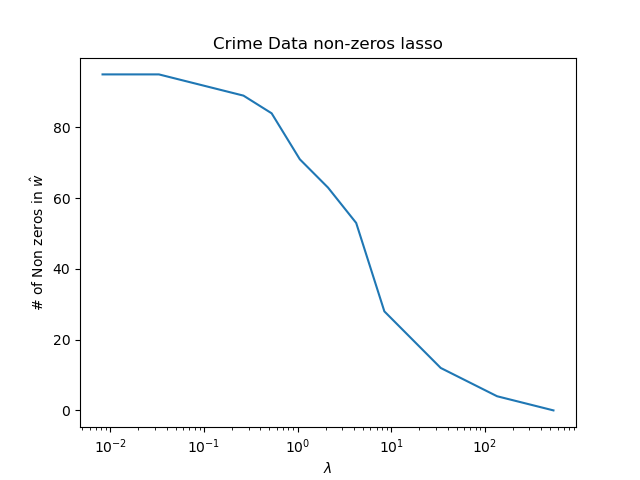
\includegraphics[width=10cm]{A5a-plot.png}
        \end{center}
    \subsection*{A.5.d}
        This is the regularization path: 
        \begin{center}
            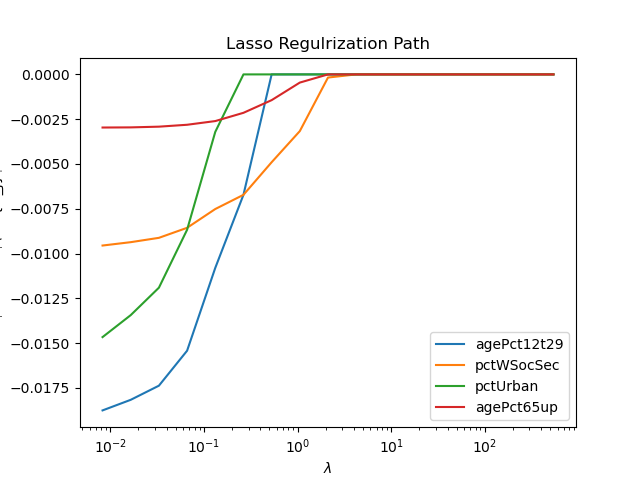
\includegraphics[width=10cm]{A5d-plot.png}
        \end{center}
    \subsection*{A.5.e}
        The error increases as the size of the regularization parameters increases. 
        \\
        Here is the plot: 
        \begin{center}
            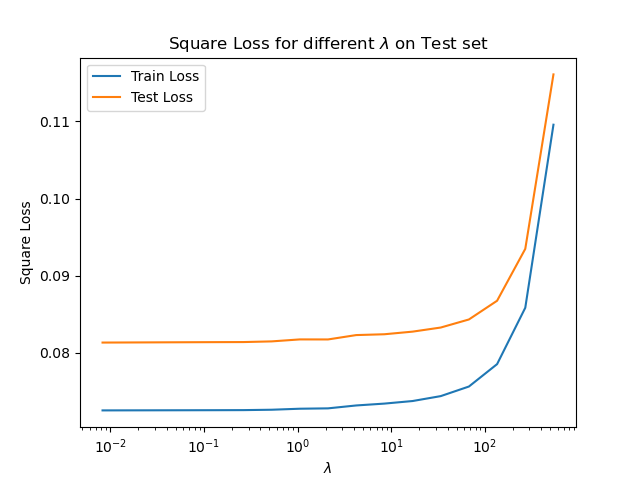
\includegraphics[width=10cm]{A5e-plot.png }
        \end{center}
    \subsection*{A.5.f}
        At a value of $\lambda = 30$, the largest lasso coefficients is identified to be: ``NumIlleg'' at a value of:  ``0.06872529'', which is: ``number of kids born to never married ''
        \\
        The smallest (Most negative) model parameters were identified to be: ``PctFam2Par'', at a value of  ``-0.06921581'', which is: ``percentage of families (with kids) that are headed by two parents''. 
    \subsection*{A.5.g}
        The politicians falsely thinks that, the cause of crime rate is because there are too many young people upon seeing the negative weights placed on ``agePct65Up'', the key here is that, \textbf{correlations doesn't imply casuality}. Every statisticians know thi. 
    \subsection*{A.5.code}
        filename: ``crime_data_lasso.py''
        file content: 
        \begin{lstlisting}
            ### Name: Hongda Alto Li
### Class: CSE 546
### This is for A5 of the HW2.
### Don't copy my code this is my code it has my style in it.

from lasso import LassoRegression, np, LassoLambdaMax
import pandas as pd
import matplotlib.pyplot as plt


def PrepareData():
    def ReadAndGet(fname):
        df = pd.read_table(fname)
        y = df["ViolentCrimesPerPop"].to_numpy()
        X = df.loc[:, df.columns != "ViolentCrimesPerPop"].to_numpy()
        print(f"{'='*10} File name: {fname} {'='*10}")
        print("Features set summary")
        print(df.loc[:, df.columns != "ViolentCrimesPerPop"].info())
        print("Labels set summary")
        print(df["ViolentCrimesPerPop"])
        print("features are already standardized. ")
        return X, y, df
    Xtrain, Ytrain, TrainDf = ReadAndGet("crime-train.txt")
    Xtest, Ytest, TestDf = ReadAndGet("crime-test.txt")
    return Xtrain, Xtest, Ytrain, Ytest, TrainDf, TestDf


def A5PlotsAndShow():
    print("summary on the data: ")
    Xtrain, Xtest, Ytrain, Ytest, TrainDf, TestDf = PrepareData()
    def A5c():
        print(f"{'='*10} Running A5(c), lambda non zeros count {'='*10}")
        LambdaMax = LassoLambdaMax(Xtrain, Ytrain)
        Lambda = LambdaMax                  # Results
        Lambdas = []                        # Results
        Ws = []                             # Predictors list
        Model = None                        # The model
        FlagPre, FlagCur = False, False     # whether lambda is < 0.01
        while (FlagPre) or (not FlagCur):   # not the case that Preivious is > 0.01, current is < 0.01
            print(f"Using Lambda: {Lambda}")
            FlagPre = FlagCur
            FlagCur = Lambda < 0.01         # Last one!
            if Model is None:
                Model = LassoRegression(regularization_lambda=Lambda)
            else:
                Model.Lambda = Lambda
            Model.fit(Xtrain, Ytrain)
            Ws.append(Model.w)
            Lambdas.append(Lambda)
            Lambda /= 2
        NoneZerosCount = [sum(_ != 0) for _ in Ws]
        plt.plot(Lambdas, NoneZerosCount)
        plt.xscale("log")
        plt.title("Crime Data non-zeros lasso")
        plt.xlabel("$\\lambda$")
        plt.ylabel("# of Non zeros in $\hat{w}$")
        plt.savefig("A5a-plot.png")
        plt.show()
        return Ws, Lambdas
    Ws, Lambdas = A5c()

    def A5d():
        # Features to pick up: agePct12t29,pctWSocSec,pctUrban,agePct65up
        Features = ["agePct12t29","pctWSocSec","pctUrban","agePct65up"]
        FeaturesIndices = []
        for II, Feature in enumerate(TrainDf.columns):
            if Feature in Features: FeaturesIndices.append(II)
        FeaturesLassoPath = np.array([w[FeaturesIndices, ...].reshape(-1) for w in Ws])
        for II in range(4):
            plt.plot(Lambdas, FeaturesLassoPath[:, II])
        plt.legend(Features)
        plt.xlabel("$\\lambda$")
        plt.ylabel("$value of $\\hat{w_j}$")
        plt.xscale("log")
        plt.title("Lasso Regulrization Path")
        plt.savefig("A5d-plot.png")
        plt.show()
    A5d()

    def A5e():
        print(f"{'='*10} Running A5(e), plotting the Squared Errors {'='*10}")
        X = Xtest[np.newaxis, ...]
        y = Ytest[np.newaxis, ...]
        y = y[..., np.newaxis]                         # 1 x n x 1
        Ws_local = np.array(Ws) # 1 x d x m
        SquareLoss = np.mean((X @ Ws_local - y) ** 2, axis=1).reshape(-1)
        plt.plot(Lambdas, SquareLoss)
        plt.title("Square Loss for different $\\lambda$ on Test set")
        plt.xlabel("$\\lambda$")
        plt.ylabel("Square Loss")
        plt.xscale("log")
        plt.savefig("A5e-plot.png")
        plt.show()

    A5e()

    def A5f():
        print(f"{'='*10} Max, mean Model Parameters {'='*10}")
        Lambda = 30
        Model  = LassoRegression(regularization_lambda=Lambda)
        Model.fit(Xtrain, Ytrain)
        w = Model.w
        WLargestIndx = np.argmax(w)
        WSmallestIdx = np.argmin(w)
        print(f"Features with the largest Lasso Coefficient is: {TrainDf.columns[WLargestIndx]}")
        print(f"Features with the smallest Lasso Coefficient is: {TrainDf.columns[WSmallestIdx]}")
        print(f"The largest value is: {w[WLargestIndx, ...]}")
        print(f"The smallest value is: {w[WSmallestIdx, ...]}")
    A5f()


def main():
    A5PlotsAndShow()


if __name__ == "__main__":
    import os
    print(f"script running at: {os.curdir}")
    print(f"cwd: {os.getcwd()}")
    print(f"script is ready to run")
    main()
        \end{lstlisting}
        
    
        
\section*{A.6}
    

\end{document}
